\actTitle{4.2 - Trigonometric Functions Defined on the Unit Circle}

\videoLink{Section 4.2 day 1}{https://www.youtube.com/playlist?list=PLYHZK3b8UFw2_C72_BEthTH-k3sKuNAEb}
%\videoLink{Section 4.2 day 2}{https://www.youtube.com/playlist?list=PLYHZK3b8UFw1pcxMutFvlZct58eGZRjlC}

\noindent \textbf{Topics:}  unit circle, trigonometric functions, trigonometric identities, periodic\\

\noindent \textbf{Student Learning Outcomes:}
\begin{enumerate}
\item Students will be able to evaluate trigonometric functions using the unit circle.
\item Students will be able to determine domains of trigonometric functions.
\item Students will be able to use trigonometric identities.
\end{enumerate}

\hrule 

\bigskip

\subsection{Pythagorean Identities} ~

$$\sin^2(t)+\cos^2(t)=1 \quad \quad \tan^2(t)+1=\sec^2(t) \quad \quad 1+\cot^2(t)=\csc^2(t)$$
\\
\begin{enumerate}
\item Given that $\tan(t)=\frac{12}{5}$ for $\pi < t < \frac{3\pi}{2}$, use an appropriate identity to find the value of $\sec(t)$.\\[2in]

\item Given that $\csc(t)=\frac{5}{4}$ for $\frac{\pi}{2} < t < \pi$, use an appropriate identity to find the value of $\cot(t)$.\\[2in]

\item Given a real number $t$, express $\sin(t)$ in terms of $\cos(t)$.\\[1.5in]

\newpage

\subsection{Even, Odd, and Periodic Properties} ~

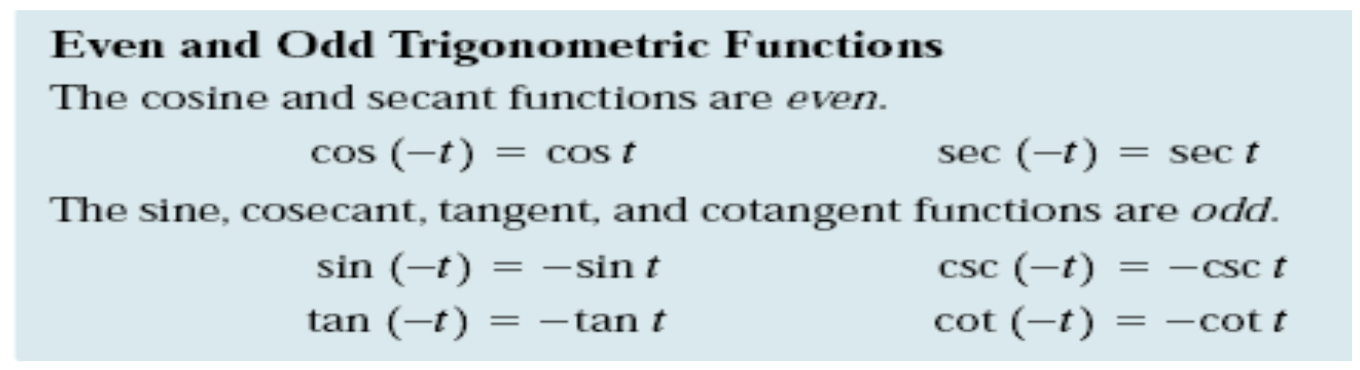
\includegraphics[scale=.6]{evenodd}\\
\item Use the unit circle to find the value of $\displaystyle \cos \Bigg(\frac{2\pi}{3}\Bigg)$ and odd trig functions to find the value of $\displaystyle \cos \Bigg(-\frac{2\pi}{3}\Bigg)$.

\vfill
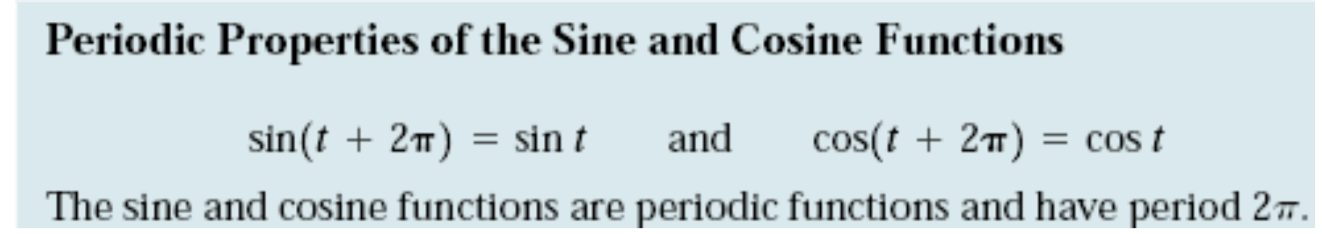
\includegraphics[scale=.6]{periodic1}\\
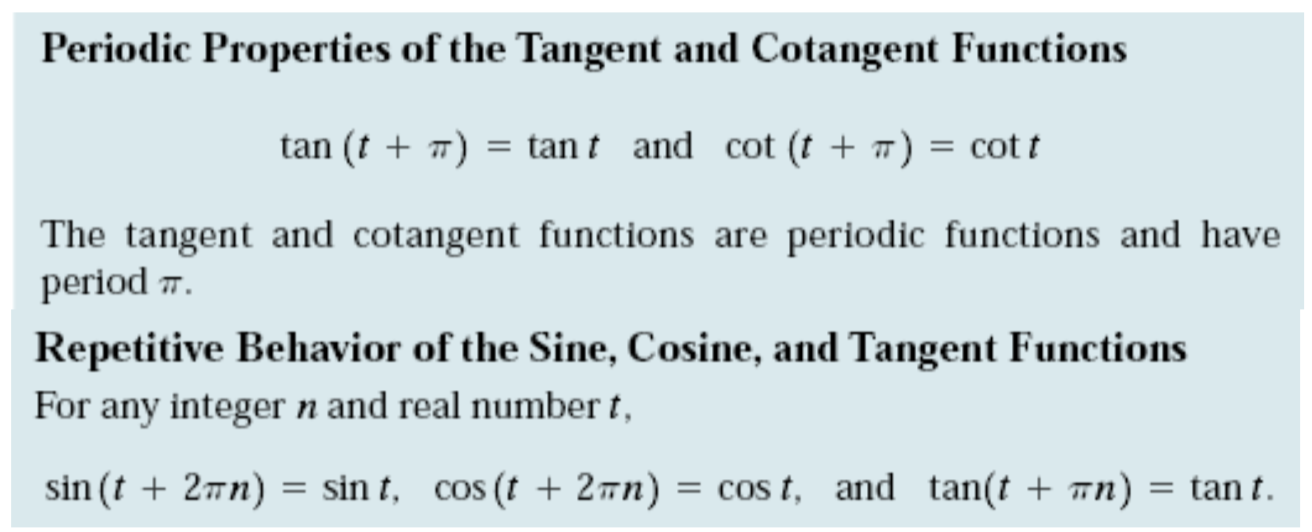
\includegraphics[scale=.6]{periodic}\\

\newpage
\item Given $\displaystyle \sin\Bigg(\frac{\pi}{12}\Bigg)=\frac{\sqrt{6}-\sqrt{2}}{4}$, determine the value of $\displaystyle \sin \Bigg( \frac{49\pi}{12} \Bigg)$.

\vfill
\item Use properties of trigonometric functions to simplify $\tan(-3t)-\tan(-3t+\pi)$.
\vfill

\subsection{Approximate Trigonometric Functions on a Calculator} ~

\item Use a calculator to approximate the function values.  Round to 4 decimal places.
\begin{enumerate}
\item $\displaystyle \cos \Bigg( \frac{2\pi}{7} \Bigg)$\\
\item $\csc(0.92)$\\[.2in]
\end{enumerate}



\end{enumerate}

\noindent \textbf{Student Learning Outcomes Check}

\begin{enumerate}
\item Can you evaluate trigonometric functions using the unit circle?
\item Can you determine domains of trigonometric functions?
\item Are you able to use trigonometric identities?

\end{enumerate}

\noindent \textbf{If any of your answers were no, please ask about these topics in class.}


